%%%%%%%%%%%%%%%%%
% This is an example CV created using altacv.cls (v1.1.3, 30 April 2017) written by
% LianTze Lim (liantze@gmail.com), based on the 
% Cv created by BusinessInsider at http://www.businessinsider.my/a-sample-resume-for-marissa-mayer-2016-7/?r=US&IR=T
% 
%% It may be distributed and/or modified under the
%% conditions of the LaTeX Project Public License, either version 1.3
%% of this license or (at your option) any later version.
%% The latest version of this license is in
%%    http://www.latex-project.org/lppl.txt
%% and version 1.3 or later is part of all distributions of LaTeX
%% version 2003/12/01 or later.
%%%%%%%%%%%%%%%%

%% If you want to use \orcid or the
%% academicons icons, add "academicons"
%% to the \documentclass options. 
%% Then compile with XeLaTeX or LuaLaTeX.
% \documentclass[10pt,a4paper,academicons]{altacv}

%% Use the "normalphoto" option if you want a normal photo instead of cropped to a circle
% \documentclass[10pt,a4paper,normalphoto]{altacv}

\documentclass[10pt,a4paper]{altacv}

%% AltaCV uses the fontawesome and academicon fonts
%% and packages. 
%% See texdoc.net/pkg/fontawecome and http://texdoc.net/pkg/academicons for full list of symbols.
%% When using the "academicons" option,
%% Compile with LuaLaTeX for best results. If you
%% want to use XeLaTeX, you may need to install
%% Academicons.ttf in your operating system's font %% folder.


% Change the page layout if you need to
\geometry{left=1cm,right=9cm,marginparwidth=6.8cm,marginparsep=1.2cm,top=1cm,bottom=1cm}

% Change the font if you want to.

% If using pdflatex:
\usepackage[utf8]{inputenc}
\usepackage[T1]{fontenc}
\usepackage[default]{lato}
\usepackage{graphics}
\usepackage{graphicx}
\usepackage[dvipsnames]{xcolor}


% If using xelatex or lualatex:
% \setmainfont{Lato}

% Change the colours if you want to
\definecolor{VividPurple}{HTML}{3E0097}
\definecolor{SlateGrey}{HTML}{2E2E2E}
\definecolor{LightGrey}{HTML}{666666}
\colorlet{heading}{VividPurple}
\colorlet{accent}{VividPurple}
\colorlet{emphasis}{SlateGrey}
\colorlet{body}{LightGrey}
\usepackage{enumerate}
\usepackage{hyperref}

\hypersetup{
    colorlinks=true,
    linkcolor=blue,
    filecolor=magenta,      
    urlcolor=darkblue,
    pdfpagemode=FullScreen,
    }
% Change the bullets for itemize and rating marker
% for \cvskill if you want to
\renewcommand{\itemmarker}{{\small\textbullet}}
\renewcommand{\ratingmarker}{\faCircle}

%% sample.bib contains your publications
\addbibresource{sample.bib}

\begin{document}
\name{Rohit Kumar}
% 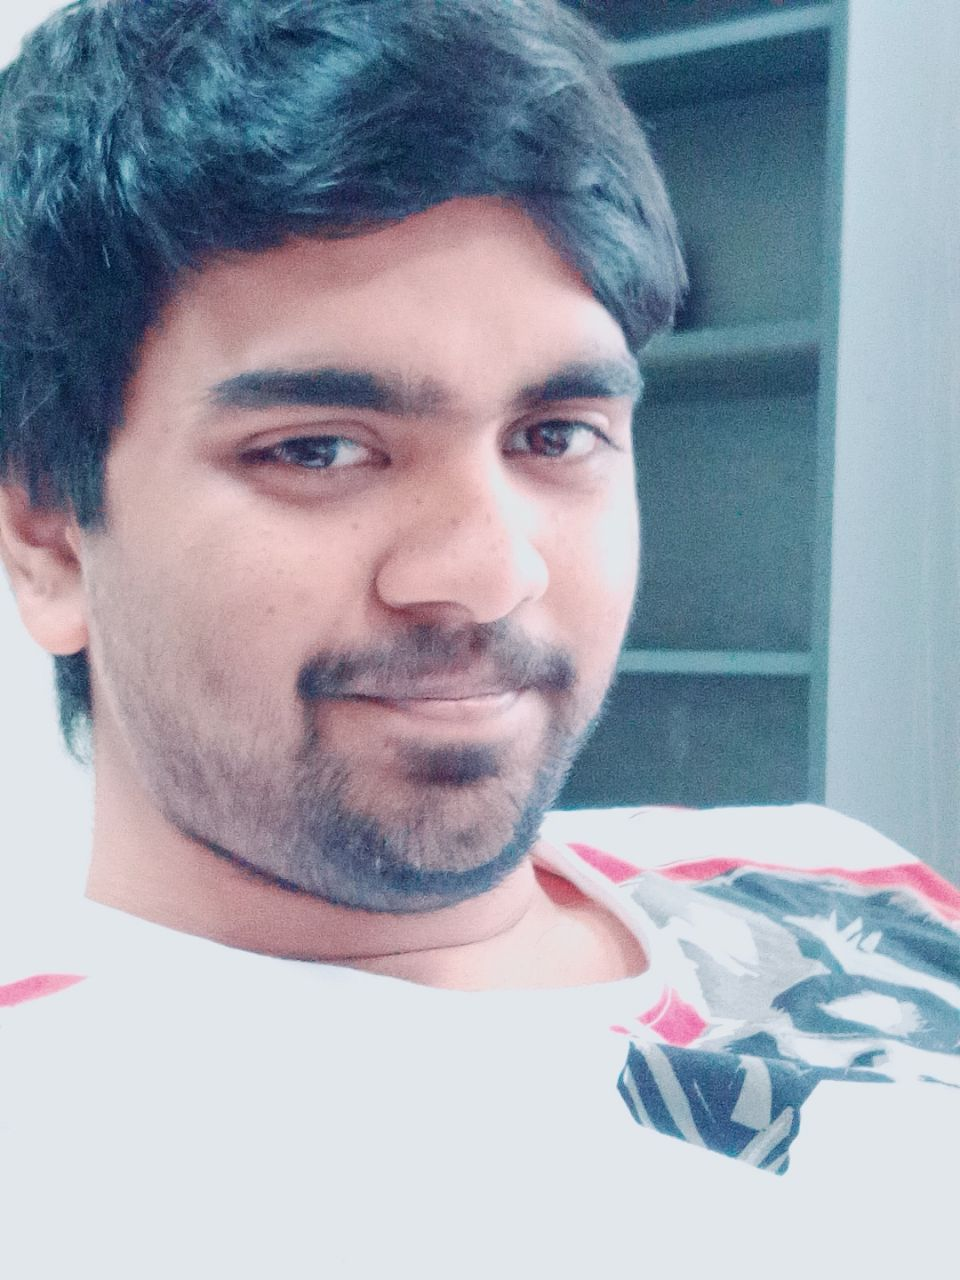
\includegraphics[width=3cm, height=4cm]{rohit}
% \tagline{Pursuing Master's in Advanced Computer Science}
\tagline{Aspiring Full Stack Developer with Expertise in Front-end Technologies}
% \photo{2.5cm}{}
\personalinfo{%
  % Not all of these are required!
  % You can add your own with \printinfo{symbol}{detail}
  \email{\href{mailto:rohitkumar93jkrs@gmail.com?subject=Greetings Rohit!&body=Hi,I found your resume and I would like to connect with you! }{rohitkumar93jkrs@gmail.com}}
  \phone{\href{tel:+447760910248}{+44 7760910248}}
  \location{\href{https://goo.gl/maps/xqTr6tpXEbRH7P1m6}{Accomb, York}}
  \linkedin{ \href{http://www.overleaf.com}{linkedin.com/in/rohitkumar93}}
  \website{\href{https://trelos.in}{Trelos.in}}
%   \github{github.com/mmayer} % I'm just making this up though.
%   \orcid{orcid.org/0000-0000-0000-0000} % Obviously making this up too. If you want to use this field (and also other academicons symbols), add "academicons" option to \documentclass{altacv}
}

%% Make the header extend all the way to the right, if you want.
\begin{fullwidth}
\makecvheader
\end{fullwidth}

%% Provide the file name containing the sidebar contents as an optional parameter to \cvsection.
%% You can always just use \marginpar{...} if you do
%% not need to align the top of the contents to any
%% \cvsection title in the "main" bar.
\cvsection[page1sidebar]{Experience}
\cvevent{Senior Software Engineer}{{Tech Mahindra}}{Sep 19 - Jul 21}{Bengaluru}
\begin{quote}
  ``Worked on a Dashboarding enterprise suite for Telecommunications market. Responsibilities included backend and frontend tasks in agile methodology and Scrum master``
\end{quote}
\begin{itemize}
\item Added several new features based on the previous architecture, now working on an Angular FastAPI Microservices API architecture with docker. Responsible for any UI or backend logic changes
\end{itemize}

\divider

\cvevent{Lead Product Developer/UI Lead}{Yantraksh Logistics Pvt. Ltd.}{Dec 18 - Sep 19}{Gurgaon}
% \cvevent{Product Developer \& UI Lead}{Cogneau Systems}{Oct 2017 -- Jul 2018}{Gurgaon}

\begin{quote}
  ``Created an ERP Supply chain automation software which reduces the cost of logistics using various optimization techniques like 3D bin-packing,Route Optimization, Fleet Allocator``
\end{quote}
\begin{itemize}
\item Created front end on react and backend on Django DRF for optimal performance
\item Deployed the app on the cloud(Google Cloud Platform) with necassary tweaks for smooth running of services along with full technical documentation of the product
\item Created automated bots to scrape large amounts of data using selenium and excel in python, for later usage or to find the current live figure
\end{itemize}

\divider

\cvevent{Lead Product Developer/UI Lead}{Cogneau Systems}{Oct 2017 -- Jul 2018}{Gurgaon}


\begin{quote}
  ``Verdis is an AI web-app made in AnguarJS which gives actionable insights about supply chain management along with full end to end visibility'
\end{quote}
\begin{itemize}

\item Created the app from scratch after 7 re-runs and finding the best amalgamation of technologies, with over 50 data visualization tools
\item Hire/train relevant talent, and lead them to meet project deadlines
\item Received 'Employee of the Year' award (Amazon Alexa™) for meeting tough milestones in short amount of time
\end{itemize}

\divider

\cvevent{Web Developer}{GreenSparrow}{Jan 2016 -- Sep 2017}{Gurgaon}

\begin{quote}
  ``Greensparrow is a division of a Silicon Valley based company called \href {www.Webenertia.com} which creates top quality websites and web-apps for US-only Clients
\end{quote}
\begin{itemize}
\item Performed complete post- and pre-launch website analysis on nearly 200 devices, and various online tests to maximize optimization whilst preserving quality standards
\end{itemize}


% \divider


% \begin{itemize}
% \item Joined the company as employe \#20 and female employee \#1
% \item Developed targeted advertisement in order to use user's search queries and show them related ads
% \end{itemize}

% \cvsection{Technologies/Skills}
% \begin{itemize}
% \item Currently learning from online courses: Python, Pandas,scikit, numpy, statistics, SQL,Data analysis algorirthms,Tensorflow
% \item Certified program in HTML, HTML5, CSS, CSS3, JavaScript,AngularJS, MySqL, Jquery,AJAX,JSON,BootStrap and PHP from CMC academy T.C.S.
% \item Microsoft Office,Adobe Photoshop, Illustrator, DreamWeaver,Sketch,ScreamFrog
% \item Slack,GIT,Basecamp,Snagit,Mamp,xamp,Phpstorm,Netbeans,Sublimetext and Trello
% \item Excellent communication skills, great synergy to work in teams, very honest personality
% \end{itemize}

%% If the NEXT page doesn't start with a \cvsection but you'd
%% still like to add a sidebar, then use this command on THIS
%% page to add it. The optional argument lets you pull up the 
%% sidebar a bit so that it looks aligned with the top of the
%% main column.
% \addnextpagesidebar[-1ex]{page3sidebar}

\endcsname
\end{document}
